\chapter{拓扑能带论}

本节要讨论的系统和\autoref{chap:conventional-metal}的哈密顿量基本上是差不多的:系统的基本自由度是某种电子,可以完全使用能带理论刻画它,相互作用可以忽略。
然而,特殊的拓扑性质会让这些系统展现出和普通的金属、绝缘体非常不同的行为。

一个典型的例子是所谓\concept{拓扑绝缘体}。
能带绝缘体中化学势位于两条能带中间,因此有明确的、彼此之间不连续的价带和导带,换而言之,载流子存在能隙(见\autoref{sec:conductor-classification})。另一方面,导体中载流子不存在能隙。
单电子能谱是否存在能隙也决定了\emph{电子态}具有或者不具有能隙,因为多电子态能够发生的最小偏移就是多一个或者少一个电子。

既然连续地、局域地调节哈密顿量不会改变能隙的有无,我们可以据此定义一个拓扑等价类。
一种比较粗糙的
% TODO:平庸芯能带
所有的传统绝缘体(就是\autoref{chap:conventional-metal}中出现的那些)都可以归入一类,这个类别中也包括真空,因为真空中的电子同样可以认为有一个价带(电子)和一个满带(正电子),两者之间存在能隙。

\begin{back}{哈密顿量的拓扑分类}{hamiltonian-topological-calssification}
    哈密顿量变化,系统的基态和激发态也会随之变化。哈密顿量的局域、连续的变化\emph{不能}让基态和激发态遍历所有的可能。
    例如,基态和激发态之间是否存在能隙这件事在哈密顿量的连续局域变化下是不会变的。
    这些诸如能隙有无之类的东西可以看成拓扑不变量,据此我们可以对哈密顿量做拓扑分类。
\end{back}

\section{Su-Schrieffer-Heeger模型}

\concept{Su-Schrieffer-Heeger(SSH)模型}是一个定义在一维格子上的紧束缚模型,在这个一维格子中有A和B两套子格。
与之前不同,我们取开放边界条件,SSH模型为
\begin{equation}
    H = v \sum_{m=1}^N (c^\dagger_{m \text{A}} c_{m \text{B}} + \text{h.c.}) + w \sum_{m=1}^{N-1} (c^\dagger_{m+1, \text{A}} c_{m \text{B}} +  \text{h.c.}).
    \label{eq:ssh-hamiltonian}
\end{equation}
我们忽略了自旋指标,即只考虑一种自旋的电子,忽略自旋翻转的可能性;使用实际的分子实现SSH模型时,会得到两份SSH模型,我们只考虑其中一份。

在分析SSH模型时通常将电子在A、B子格上的哪一个看成内禀自由度而非坐标自由度或者说外部自由度,这实际上就是紧束缚模型中把能带标签当成抽象的一个指标而忽略它对电子空间分布的影响,而将$\vb*{i}$看成完全代表了电子空间位置的标签的做法。
在这种约定下,\eqref{eq:ssh-hamiltonian}可以写成
\begin{equation}
    H = v \sum_{m=1}^N \dyad{m} \otimes \sigma^x + w \sum_{m=1}^{N-1} \dyad{m+1}{m} \otimes \frac{\sigma^x + \ii \sigma^y}{2} + \text{h.c.}. 
\end{equation}

\begin{figure}
    \centering
    

\tikzset{every picture/.style={line width=0.75pt}} %set default line width to 0.75pt        

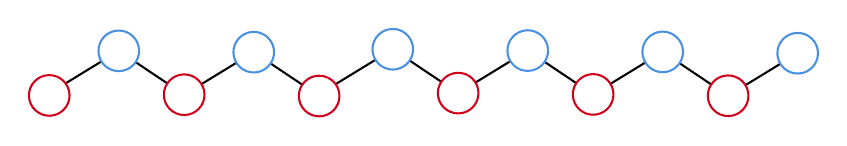
\begin{tikzpicture}[x=0.75pt,y=0.75pt,yscale=-1,xscale=1]
%uncomment if require: \path (0,300); %set diagram left start at 0, and has height of 300

%Straight Lines [id:da5978907907830429] 
\draw    (101.11,108.45) -- (132.62,129.57) ;
%Straight Lines [id:da6479636898097754] 
\draw    (166.14,109.09) -- (197.65,130.21) ;
%Straight Lines [id:da20799022198939388] 
\draw    (233.12,107.68) -- (264.64,128.81) ;
%Straight Lines [id:da7588059918995707] 
\draw    (298.15,108.32) -- (329.66,129.45) ;
%Straight Lines [id:da04554146426034689] 
\draw    (363.18,108.96) -- (394.69,130.09) ;
%Straight Lines [id:da6866628962323054] 
\draw    (67.6,128.94) -- (101.11,108.45) ;
%Shape: Circle [id:dp960424577904551] 
\draw  [color={rgb, 255:red, 208; green, 2; blue, 27 }  ,draw opacity=1 ][fill={rgb, 255:red, 255; green, 255; blue, 255 }  ,fill opacity=1 ] (57.83,130.14) .. controls (57.72,124.74) and (62.01,120.27) .. (67.41,120.15) .. controls (72.82,120.04) and (77.29,124.33) .. (77.4,129.73) .. controls (77.51,135.13) and (73.23,139.61) .. (67.82,139.72) .. controls (62.42,139.83) and (57.95,135.54) .. (57.83,130.14) -- cycle ;
%Shape: Circle [id:dp278517736754311] 
\draw  [color={rgb, 255:red, 74; green, 144; blue, 226 }  ,draw opacity=1 ][fill={rgb, 255:red, 255; green, 255; blue, 255 }  ,fill opacity=1 ] (91.32,108.65) .. controls (91.21,103.25) and (95.5,98.78) .. (100.9,98.67) .. controls (106.31,98.55) and (110.78,102.84) .. (110.89,108.24) .. controls (111.01,113.65) and (106.72,118.12) .. (101.31,118.23) .. controls (95.91,118.35) and (91.44,114.06) .. (91.32,108.65) -- cycle ;
%Straight Lines [id:da8951114155214333] 
\draw    (132.62,129.57) -- (166.14,109.09) ;
%Shape: Circle [id:dp6119193772576137] 
\draw  [color={rgb, 255:red, 208; green, 2; blue, 27 }  ,draw opacity=1 ][fill={rgb, 255:red, 255; green, 255; blue, 255 }  ,fill opacity=1 ] (122.84,129.78) .. controls (122.73,124.38) and (127.02,119.9) .. (132.42,119.79) .. controls (137.82,119.68) and (142.29,123.97) .. (142.41,129.37) .. controls (142.52,134.77) and (138.23,139.25) .. (132.83,139.36) .. controls (127.43,139.47) and (122.95,135.18) .. (122.84,129.78) -- cycle ;
%Shape: Circle [id:dp7508217961101133] 
\draw  [color={rgb, 255:red, 74; green, 144; blue, 226 }  ,draw opacity=1 ][fill={rgb, 255:red, 255; green, 255; blue, 255 }  ,fill opacity=1 ] (156.35,109.29) .. controls (156.24,103.89) and (160.53,99.42) .. (165.93,99.3) .. controls (171.33,99.19) and (175.81,103.48) .. (175.92,108.88) .. controls (176.03,114.29) and (171.74,118.76) .. (166.34,118.87) .. controls (160.94,118.98) and (156.47,114.7) .. (156.35,109.29) -- cycle ;
%Straight Lines [id:da6824105788244417] 
\draw    (199.61,128.17) -- (233.12,107.68) ;
%Shape: Circle [id:dp6550057353578134] 
\draw  [color={rgb, 255:red, 208; green, 2; blue, 27 }  ,draw opacity=1 ][fill={rgb, 255:red, 255; green, 255; blue, 255 }  ,fill opacity=1 ] (187.87,130.42) .. controls (187.75,125.01) and (192.04,120.54) .. (197.45,120.43) .. controls (202.85,120.32) and (207.32,124.6) .. (207.43,130.01) .. controls (207.55,135.41) and (203.26,139.88) .. (197.86,140) .. controls (192.45,140.11) and (187.98,135.82) .. (187.87,130.42) -- cycle ;
%Shape: Circle [id:dp2789113887024053] 
\draw  [color={rgb, 255:red, 74; green, 144; blue, 226 }  ,draw opacity=1 ][fill={rgb, 255:red, 255; green, 255; blue, 255 }  ,fill opacity=1 ] (223.34,107.89) .. controls (223.22,102.49) and (227.51,98.01) .. (232.92,97.9) .. controls (238.32,97.79) and (242.79,102.08) .. (242.9,107.48) .. controls (243.02,112.88) and (238.73,117.35) .. (233.33,117.47) .. controls (227.92,117.58) and (223.45,113.29) .. (223.34,107.89) -- cycle ;
%Straight Lines [id:da9835803759861903] 
\draw [color={rgb, 255:red, 0; green, 0; blue, 0 }  ,draw opacity=1 ][fill={rgb, 255:red, 208; green, 2; blue, 27 }  ,fill opacity=1 ]   (264.64,128.81) -- (298.15,108.32) ;
%Shape: Circle [id:dp3465061446468005] 
\draw  [color={rgb, 255:red, 208; green, 2; blue, 27 }  ,draw opacity=1 ][fill={rgb, 255:red, 255; green, 255; blue, 255 }  ,fill opacity=1 ] (254.85,129.02) .. controls (254.74,123.61) and (259.03,119.14) .. (264.43,119.03) .. controls (269.83,118.91) and (274.31,123.2) .. (274.42,128.61) .. controls (274.53,134.01) and (270.24,138.48) .. (264.84,138.59) .. controls (259.44,138.71) and (254.97,134.42) .. (254.85,129.02) -- cycle ;
%Shape: Circle [id:dp2919589177523425] 
\draw  [color={rgb, 255:red, 74; green, 144; blue, 226 }  ,draw opacity=1 ][fill={rgb, 255:red, 255; green, 255; blue, 255 }  ,fill opacity=1 ] (288.36,108.53) .. controls (288.25,103.12) and (292.54,98.65) .. (297.94,98.54) .. controls (303.35,98.43) and (307.82,102.71) .. (307.93,108.12) .. controls (308.05,113.52) and (303.76,117.99) .. (298.35,118.11) .. controls (292.95,118.22) and (288.48,113.93) .. (288.36,108.53) -- cycle ;
%Straight Lines [id:da3388603264007448] 
\draw    (329.66,129.45) -- (363.18,108.96) ;
%Shape: Circle [id:dp22822608286568746] 
\draw  [color={rgb, 255:red, 208; green, 2; blue, 27 }  ,draw opacity=1 ][fill={rgb, 255:red, 255; green, 255; blue, 255 }  ,fill opacity=1 ] (319.88,129.65) .. controls (319.77,124.25) and (324.06,119.78) .. (329.46,119.66) .. controls (334.86,119.55) and (339.33,123.84) .. (339.45,129.24) .. controls (339.56,134.65) and (335.27,139.12) .. (329.87,139.23) .. controls (324.47,139.35) and (319.99,135.06) .. (319.88,129.65) -- cycle ;
%Shape: Circle [id:dp9731435281234146] 
\draw  [color={rgb, 255:red, 74; green, 144; blue, 226 }  ,draw opacity=1 ][fill={rgb, 255:red, 255; green, 255; blue, 255 }  ,fill opacity=1 ] (353.39,109.17) .. controls (353.28,103.76) and (357.57,99.29) .. (362.97,99.18) .. controls (368.37,99.06) and (372.85,103.35) .. (372.96,108.76) .. controls (373.07,114.16) and (368.78,118.63) .. (363.38,118.74) .. controls (357.98,118.86) and (353.51,114.57) .. (353.39,109.17) -- cycle ;
%Straight Lines [id:da7953208412330044] 
\draw    (394.69,130.09) -- (428.2,109.6) ;
%Shape: Circle [id:dp6293699664956078] 
\draw  [color={rgb, 255:red, 208; green, 2; blue, 27 }  ,draw opacity=1 ][fill={rgb, 255:red, 255; green, 255; blue, 255 }  ,fill opacity=1 ] (384.91,130.29) .. controls (384.79,124.89) and (389.08,120.42) .. (394.49,120.3) .. controls (399.89,120.19) and (404.36,124.48) .. (404.48,129.88) .. controls (404.59,135.29) and (400.3,139.76) .. (394.9,139.87) .. controls (389.49,139.98) and (385.02,135.7) .. (384.91,130.29) -- cycle ;
%Shape: Circle [id:dp5339722494647174] 
\draw  [color={rgb, 255:red, 74; green, 144; blue, 226 }  ,draw opacity=1 ][fill={rgb, 255:red, 255; green, 255; blue, 255 }  ,fill opacity=1 ] (418.42,109.8) .. controls (418.31,104.4) and (422.6,99.93) .. (428,99.82) .. controls (433.4,99.7) and (437.87,103.99) .. (437.99,109.39) .. controls (438.1,114.8) and (433.81,119.27) .. (428.41,119.38) .. controls (423.01,119.5) and (418.53,115.21) .. (418.42,109.8) -- cycle ;




\end{tikzpicture}

    \caption{SSH模型所在的格点,红色和蓝色圆圈分别代表A子格和B子格,只有相邻格点之间有跃迁}
\end{figure}

\subsection{体态}

一个有限大小的一维格子的体态是其内部,而边界则是两个点。本节分析SSH模型的体态。取热力学极限$N \to \infty$并施加周期性边界条件,可以求解得到普通的能带。
做傅里叶变换
\begin{equation}
    c_{m \alpha}^\dagger = \frac{1}{\sqrt{N}} \sum_k \ee^{- \ii k m a} c_{k \alpha}^\dagger, \quad \alpha = \text{A}, \text{B},
\end{equation}
得到
\begin{equation}
    H = \sum_k \pmqty{c^\dagger_{k \text{A}} & c^\dagger_{k \text{B}}} \pmqty{ 0 & v + w \ee^{- \ii k a} \\ v + w \ee^{\ii k a} & 0 } \pmqty{ c_{k \text{A}} \\ c_{k \text{B}} },
\end{equation}
对角化给出
\begin{equation}
    \epsilon_{k} = \pm \sqrt{ v^2 + w^2 + 2 wv \cos(ka) }.
\end{equation}
两条能带之间的间距为
\begin{equation}
    2 \Delta = \abs{u - v}.
\end{equation}
容易看出在化学势为零时电子半填充,且电子和空穴的能隙(相对于费米面的距离)均为$\Delta$。

在$u=v$时我们得到通常的最为简单的紧束缚模型,系统是导体,因为载流子能隙为零;其余情况下,系统为绝缘体。
换而言之,跃迁系数的交错排列(staggering)让SSH模型是绝缘体。

\section{整数量子霍尔效应}

具有能隙的电子态同样可以因为拓扑而有非平凡的行为,典型的例子是整数量子霍尔效应。
经典霍尔效应预言的霍尔电导为\eqref{eq:classical-hall-conductivity},于是霍尔电阻正比于$B$。
然而在低温、强磁场下,观察到$\rho$和$B$之间的关系\emph{存在平台}(所谓\concept{电导平台}),稳定时的$\nu$取值为
\[
    \nu = 1, 2, 3, \cdots, \frac{1}{3}, \frac{2}{3}, \frac{2}{5}, \cdots.
\]
$\nu$取整数的情况称为\concept{整数量子霍尔效应},取分数的情况为\concept{分数量子霍尔效应}。

事实证明,整数量子霍尔效应仅仅在拓扑能带理论的框架下即可得到很好的解释,即它实质上还是一个短程纠缠系统。
分数量子霍尔效应则涉及强关联效应,而且存在拓扑序,即有长程纠缠。

\subsection{整数电导平台的定性分析}

\subsubsection{朗道能级}

在\autoref{sec:quantum-magnetic-field}中我们已经考虑过了朗道能级。
设被填充的最高的朗道能级编号为$n$,且填充在朗道能级中的电子总数为$N_\text{e}$,则有
\[
    \frac{N_\text{e}}{2} = (n-1) \frac{\Phi}{\Phi_0} + n_\text{high}, \quad 0 < n_\text{high} \leq \frac{\Phi}{\Phi_0},
\]
于是随着$1/B$上升(即$B$下降),$n$能级上的电子轨道占据数$n_\text{high}$线性上升。
如果我们能够保证电导大体上正比于电子填充数,那么以上机制就给出了电导平台的一种可能成因。

如果材料是非常理想的,那么其实不应该出现电导平台,因为此时$n$朗道能级被填充之后,立刻会开始填充$n+1$朗道能级。
然而实际的体系中有杂质,因此朗道能级会出现展宽,并且两个朗道能级之间的态基本上是局域化态,而朗道能级中的态则舒展一些(见\autoref{sec:anderson-localization})。
换而言之,朗道能级附近的电子可以自由移动,在化学势在它们附近时它们可以贡献电导,而两个朗道能级之间的电子高度定域,任何时候都无法贡献电导。
因此,在填充延展态时电导关于$1/B$线性上升,而在填充定域态时电导没有变化。
这就造成了一个非常矛盾的情况:要观察到电导平台,体系必须比较“脏”,这样才能够有明确的定域态,从而形成平台,否则,化学势可以从一个朗道能级快速跳转到另一个朗道能级,平台是看不到的。
但实际上,在体系很脏时朗道能级附近的延展态也被破坏了,因此太脏的体系展现不出太多平台。
因此明显的量子霍尔效应需要体系有些脏但又不太脏。

然而我们马上会注意到一个不对头的地方。大部分时候,化学势都不在朗道能级上,而是在两个朗道能级之间,即化学势位于能隙之中。
因此,我们实际上是在要求有能隙的电子模式——朗道能级——产生电流!
唯一的可能是,体态有能隙,但边界态没有能隙,从而边界态导电。
如果真的能够形成能导电的边界态,体态有能隙倒不是坏事,因为这意味着体态内部的关联长度有限,因此边界态和体态相对独立。

朗道能级确实能够形成稳定的边界态电流。
可以从一个经典图像看到这一点:在体态中电子可以不停做圆周运动,而在边界附近电子做完半个圆周运动后被反弹,而又往前做半个圆周运动。
因此,可以形成绕着整个边界运行的(手性的)电流。边界态上如果有杂质,电子可以潜到体态中,绕过杂质,形成一个新的边界态。因此边界态上的电流是无损耗的。

在磁场比较高时,只有几个朗道能级上面填充了电子,从而霍尔电导比较低,霍尔电阻比较高,从而能够容易地观察到量子霍尔效应。

\subsubsection{霍尔电导的形式和Laughlin论证}

然而以上论证无法解释一件事,就是为什么电导平台的值不多不少,就是几个基本物理常数确定的
\[
    \sigma_\text{H} = n \frac{e^2}{h}, \quad n = 0, 1, 2, \ldots.
\]
通常的电导涉及关于材料的复杂性质,是不可能如此简洁的。
\concept{Laughlin论证}是一种直观理解关于为什么霍尔电导形式非常简洁的方法。
设有一个半径为$L$的圆柱体,其体态有能隙而边界态导电。
沿着它的轴向加入一个磁场,总磁通量为$\Phi$。让$\Phi$缓慢地发生变化,从零变化到$\frac{h c}{e}$,则$\Phi$变化前后圆柱体均处于同样的状态,因为绕着大小为$h / e$的磁通量转一圈什么也不会发生。
磁通量的变化会导致一个电场,在边界上,我们有
\[
    2 \pi L E = - \dv{\Phi}{t},
\]
从而
\[
    E(t) = \frac{1}{2\pi L} \dv{\Phi}{t}.
\]
边界上的电场方向垂直轴向,从而产生一个平行于轴向的霍尔电流
\[
    I = 2 \pi L j = 2 \pi L \sigma_\text{H} E = {\sigma_\text{H}} \dv{\Phi}{t}.
\]
这个电流造成的电荷量变化为
\[
    \Delta Q = \int \dd{t} I = {\sigma_\text{H}} \Delta \Phi = \sigma_\text{H} \frac{h}{e},
\]
而由于电荷由电子携带,有
\[
    \Delta Q = me, \quad m = 0, 1, 2, \ldots,
\]
于是
\[
    \sigma_\text{H} = m \frac{e^2}{h}, \quad m = 0, 1, 2, \ldots.
\]
这就是整数阶量子霍尔效应的来源:它和体系的结构完全无关,只要体系体态有能隙,就能够得出存在整数霍尔效应的结论。

\subsection{线性响应理论和拓扑不变量}

以上的定性分析能够解释整数量子霍尔效应,不过我们当然想要一个更加一般的、能够适用于各种类似的系统的解释。



\begin{back}{Berry相位}{berry-phase}
    设含时哈密顿量$H$依赖一系列连续参数$\vb{R}(t) = (R_1(t), \ldots, R_n(t))$,用$\ket{n(\vb{R}(t))}$标记该哈密顿量的本征态。
    假定$\vb{R}(t)$变化得(相比于$H$的能谱的最小能隙)充分缓慢,以至于如果系统以$\ket{n(\vb{R}(t))}$为初态,那么经过一段时间的演化之后不会跃迁到其他本征态上(\concept{绝热演化})。
    
    设系统初态为$\ket{n(\vb{R}(t))}$,经过一段时间后系统状态为
    \begin{equation}
        \ket{\psi_n(t)} = \ee^{\ii \gamma_n(t)} \exp(-\frac{\ii}{\hbar} \int_0^t \dd{t'} E_n(\vb{R}(t'))) \ket{n(\vb{R}(t))},
    \end{equation}
    将上式代入
    \[
        \ii \hbar \dv{t} \ket{\psi_n(t)} = H(\vb{R}(t)) \ket{\psi_n(t)},
    \]
    得到
    \begin{equation}
        \gamma_n(t) = \ii \int_0^t \dd{t'} \mel*{\psi_n(t)}{\dv{t}}{\psi_n(t)} = \ii \int_{\vb{R}(0)}^{\vb{R}(t)} \dd{\vb{R}} \cdot \mel*{\psi_n(t)}{\grad_{\vb{R}}}{\psi_n(t)} .
    \end{equation}
    注意到$\gamma_n(t)$不含有任何$\hbar$,因此实际上这\emph{不是}一个动力学相位,而是所谓的几何相位。
    定义
    \begin{equation}
        \vb{A} = \ii \mel*{\psi_n(t)}{\grad_{\vb{R}}}{\psi_n(t)} 
    \end{equation}
    为\concept{Berry联络},相应的相位称为\concept{Berry相位}。
    这里的底流形是参数空间,其上的协变导数定义要求相邻两个$\vb{R}$对应的态可以通过绝热演化连接。
    Berry联络就是满足这个条件的联络。从Berry联络自然可以得到Berry曲率张量
    \begin{equation}
        \Omega_{n, \mu \nu} = \partial_{R_\mu} \partial_{R_\nu} A_n - \partial_{R_\nu} \partial_{R_\mu} A_n.
    \end{equation}
    
    Berry联络是规范可变的,因为容易验证,如果做变换
    \begin{equation}
        \ket{n(\vb{R})} \longrightarrow \ee^{\ii \zeta(\vb{R})} \ket{n(\vb{R})}, 
    \end{equation}
    就有
    \begin{equation}
        \vb{A}(\vb{R}) \longrightarrow \vb{A}(\vb{R}) - \grad_{\vb{R}} \zeta(\vb{R}).
    \end{equation}
    在时间从$0$演化到$T$的闭合的$\vb{R}(t)$回路上,由于单值性,有
    \[
        \zeta(\vb{R}(T)) - \zeta(\vb{R}(0)) = 2 \pi n, \quad n \in \mathbb{Z},
    \]
    从而积分
    \begin{equation}
        \oint \dd{\vb{R}} \cdot \vb{A}
    \end{equation}
    在模$2\pi$的意义下是规范不变的。

    以上讨论的问题中参数空间都是外加参数,但是实际上也可以用系统内的物理量做参数。
    现在向系统中加入一个变化缓慢的外场,用它“牵引”系统做绝热演化,由于
    因此此时$\mel{g}{\partial_t}{g}$就给出一个Berry相位,参数空间是外场的参数空间,而由于是绝热演化,外场通常会让系统中的某一些物理量非常确定,那么我们就能够用系统中的物理量做参数了。
    例如,可以在空间中假象地引入一个势阱,用它让粒子每一时刻都几乎位于一个确定的位置,则这个势阱的位置——实际上就是粒子的位置——的取值范围(比如说一圆圈)就构成了一个参数空间,其上就可以定义Berry联络。
    A-B效应就是一个典型例子,在那里参数就是粒子位置$\vb*{r}$。
    在拓扑能带论中,参数则可以是晶格动量$\vb*{k}$。

    Berry相位可以体现在路径积分中。回顾各种路径积分的推导方式,都可以找到类似于$\mel{g}{\partial_t}{g}$的项,其中$\ket{g}$通常是某种“相干态”。
    设相干态是关于某些变量$q$的,回顾路径积分的推导过程,$\mel{g}{\partial_t}{g}$项实际上就对应着经典的从哈密顿量到拉格朗日量的勒让德变换中$p \dot{q}$这一项,因此如果有非平庸的Berry相位那么它一定会被收集在这一项中。
    因此拉氏量中的$p \dot{q}$项常常被称为Berry相位项,虽然一般情况下它也会容纳一些动力学演化的信息。
    $q$高度确定的绝热演化过程中,$p$中显含$\dot{q}$的项都可以丢弃,因为演化速度很慢(实际上$\dot{q}$通常和$q$是不对易的,不过无所谓,反正都是要丢弃的),于是$\int \dd{t} p \dot{q}$可以写成$\int p(q) \dd{q}$,此时它就是Berry相位。
\end{back}

\section{一维Kitaev链拓扑超导体}

\subsection{Kitaev链及其解析解}

以下一维模型称为\concept{Kitaev链}:
\begin{equation}
    {H} = - t \sum_{i} ({c}_{i}^\dagger {c}_{i+1} + \text{h.c.}) - \mu \sum_{i} {c}_{i}^\dagger {c}_{i} + \sum_{i} (\Delta {c}_{i} {c}_{i+1} + \text{h.c.} ).
    \label{eq:kitaev-chain-hamiltonian}
\end{equation}
\eqref{eq:kitaev-chain-hamiltonian}是一个p波超导模型,这个模型通常是这么来的:一个一维纳米线被放置在一个超导体上,两者的相互作用诱导前者也发生$U(1)$对称性破缺,然后我们使用平均场理论分析问题而引入一个$\Delta$参量。
\eqref{eq:kitaev-chain-hamiltonian}是一个紧束缚模型,
对\eqref{eq:kitaev-chain-hamiltonian}做傅里叶变换,可以得到
\begin{equation}
    {H} = \frac{1}{2} \sum_{\vb*{k}} \underbrace{\pmqty{{c}^\dagger_{\vb*{k}} & {c}_{-\vb*{k}}}}_{{\Psi}^\dagger} \pmqty{\epsilon_{\vb*{k}} - \mu & -2 \ii \Delta^* \sin k \\ 2 \ii \Delta \sin k & - \epsilon_{\vb*{k}} + \mu} \underbrace{\pmqty{{c}_{\vb*{k}} \\ {c}^\dagger_{-\vb*{k}}}}_{{\Psi}},
\end{equation}
然后再做Bogoliubov变换,计算出以下能谱:
\begin{equation}
    E_{\vb*{k}} = \pm \sqrt{(2t \cos k - \mu)^2 + 4 \abs{\Delta}^2 \sin^2 k}.
\end{equation}

\eqref{eq:kitaev-chain-hamiltonian}具有粒子-空穴对称性。% TODO
总之就有一个约束就是设$P$为粒子空穴变换,我们有
\[
    P {\Psi}_{\vb*{k}} P^{-1} = \tau^* {\Psi}_{-\vb*{k}}^*
\]

Kitaev链不存在对称性自发破缺,但能隙可开可闭。当
\begin{equation}
    \mu = \pm 2t
    \label{eq:kitaev-gap-point}
\end{equation}
时,能隙会关闭。除此之外任何参数的变动都只会引起连续的变化。
因此,如果体系发生相变,那么只能是在\eqref{eq:kitaev-gap-point}处发生一个和对称性无关的相变。在化学势很低时,即$\mu$趋于负无穷时,根本就没有电子,因此从$-\infty$到$-2t$的部分肯定是平庸的。
化学势非常高时(大于$2t$时)电子全满,同样是平庸的。
因此有趣的行为集中在$-2t$到$2t$之间。下面会看到,当$\mu$越过\eqref{eq:kitaev-gap-point}这两个点时,会发生一个拓扑相变。

$W = \pm 1$,这是一个定义在立体中的量?

\subsection{Kitaev链中的拓扑不变量}

下面定义一个能带的拓扑不变量。

总之,当$\mu$扫过$\mu=-2t$时,我们有
\[
    {c}_{\vb*{i}} = \frac{1}{2} ({\gamma}_{i\text{A}} + \ii {\gamma}_{i \text{B}}),
\]
容易验证均为
\begin{equation}
    \acomm*{{\gamma}_\alpha}{{\gamma}_\beta^\dagger} = 2 \delta_{\alpha \beta},
\end{equation}

\subsection{时间反演对称性保护的拓扑超导}

刚才描述的拓扑超导和对称性没有特别明确的对称性。当然可以说它有粒子-空穴对称性,但是这完全是一个数学上的处理。